\documentclass{ximera}

%\addPrintStyle{..}

\begin{document}
	\author{Bart Lambregs}
	\xmtitle{Oefeningen kinematica}{}
    \xmsource\xmuitleg




\begin{exercise}
	Kan de snelheid van een voorwerp gelijk zijn aan nul, terwijl de versnelling verschillend is van nul? Motiveer je antwoord.
\end{exercise}


\begin{exercise}
	Kan een voorwerp dat een positieve versnelling heeft een negatieve snelheid hebben? Kan het omgekeerde ook? Licht je antwoord toe.

	\begin{oplossing}
		Ja, dat kan. Neem bijvoorbeeld een voorwerp dat je verticaal omhoog gooit. Als je de referentieas waarmee je de beweging wil beschrijven verticaal naar beneden kiest, zal de versnelling van de beweging positief zijn en de snelheid negatief. De snelheid is negatief omdat je tegengesteld aan de as beweegt en de versnelling is positief omdat de snelheid minder negatief wordt.

		Het omgekeerde kan ook, draai gewoon de referentieas om.
	\end{oplossing}
\end{exercise}

\begin{exercise}
	Een puntmassa beweegt volgens de plaatsfunctie
	\[
	x(t)=t^3-3t^2-10t
	\]
	Bereken haar snelheidscomponent telkens als ze het vertrekpunt passeert. Hoe groot is dan de versnellingscomponent?
	\begin{oplossing}
		$x=t(t-5)(t+2)$
	\end{oplossing}
\end{exercise}


\begin{exercise}
Een veerman tracht een stromende rivier loodrecht over te roeien. Hij slaagt erin ten opzicht van het water een snelheid van \SI{2,00}{m/s} te ontwikkelen -- de stroomsnelheid is \SI{1,25}{m/s}. De rivier is \SI{150}{\meter} breed. 

\begin{question}
 Onder welke hoek ten opzichte van de loodlijn op de oever moet hij steeds blijven roeien?
\begin{oplossing}
Er is gegeven dat

\begin{itemize}
	\item $v_1=\SI{2}{\meter\per\second}$
	\item$v_2=\SI{1,25}{\meter\per\second}$
	\item $d=\SI{150}{\meter}$
\end{itemize}

We berekenen de hoek $\alpha$. 


De component, tegengesteld aan de zin waarin het water stroomt, van de snelheid waarmee de veerman roeit ten opzichte van het water, moet even groot zijn als de stroomsnelheid zodat de veerman in de richting van de rivier resulterend geen snelheid zal hebben.

% \begin{figure}[h]
% \centering
% 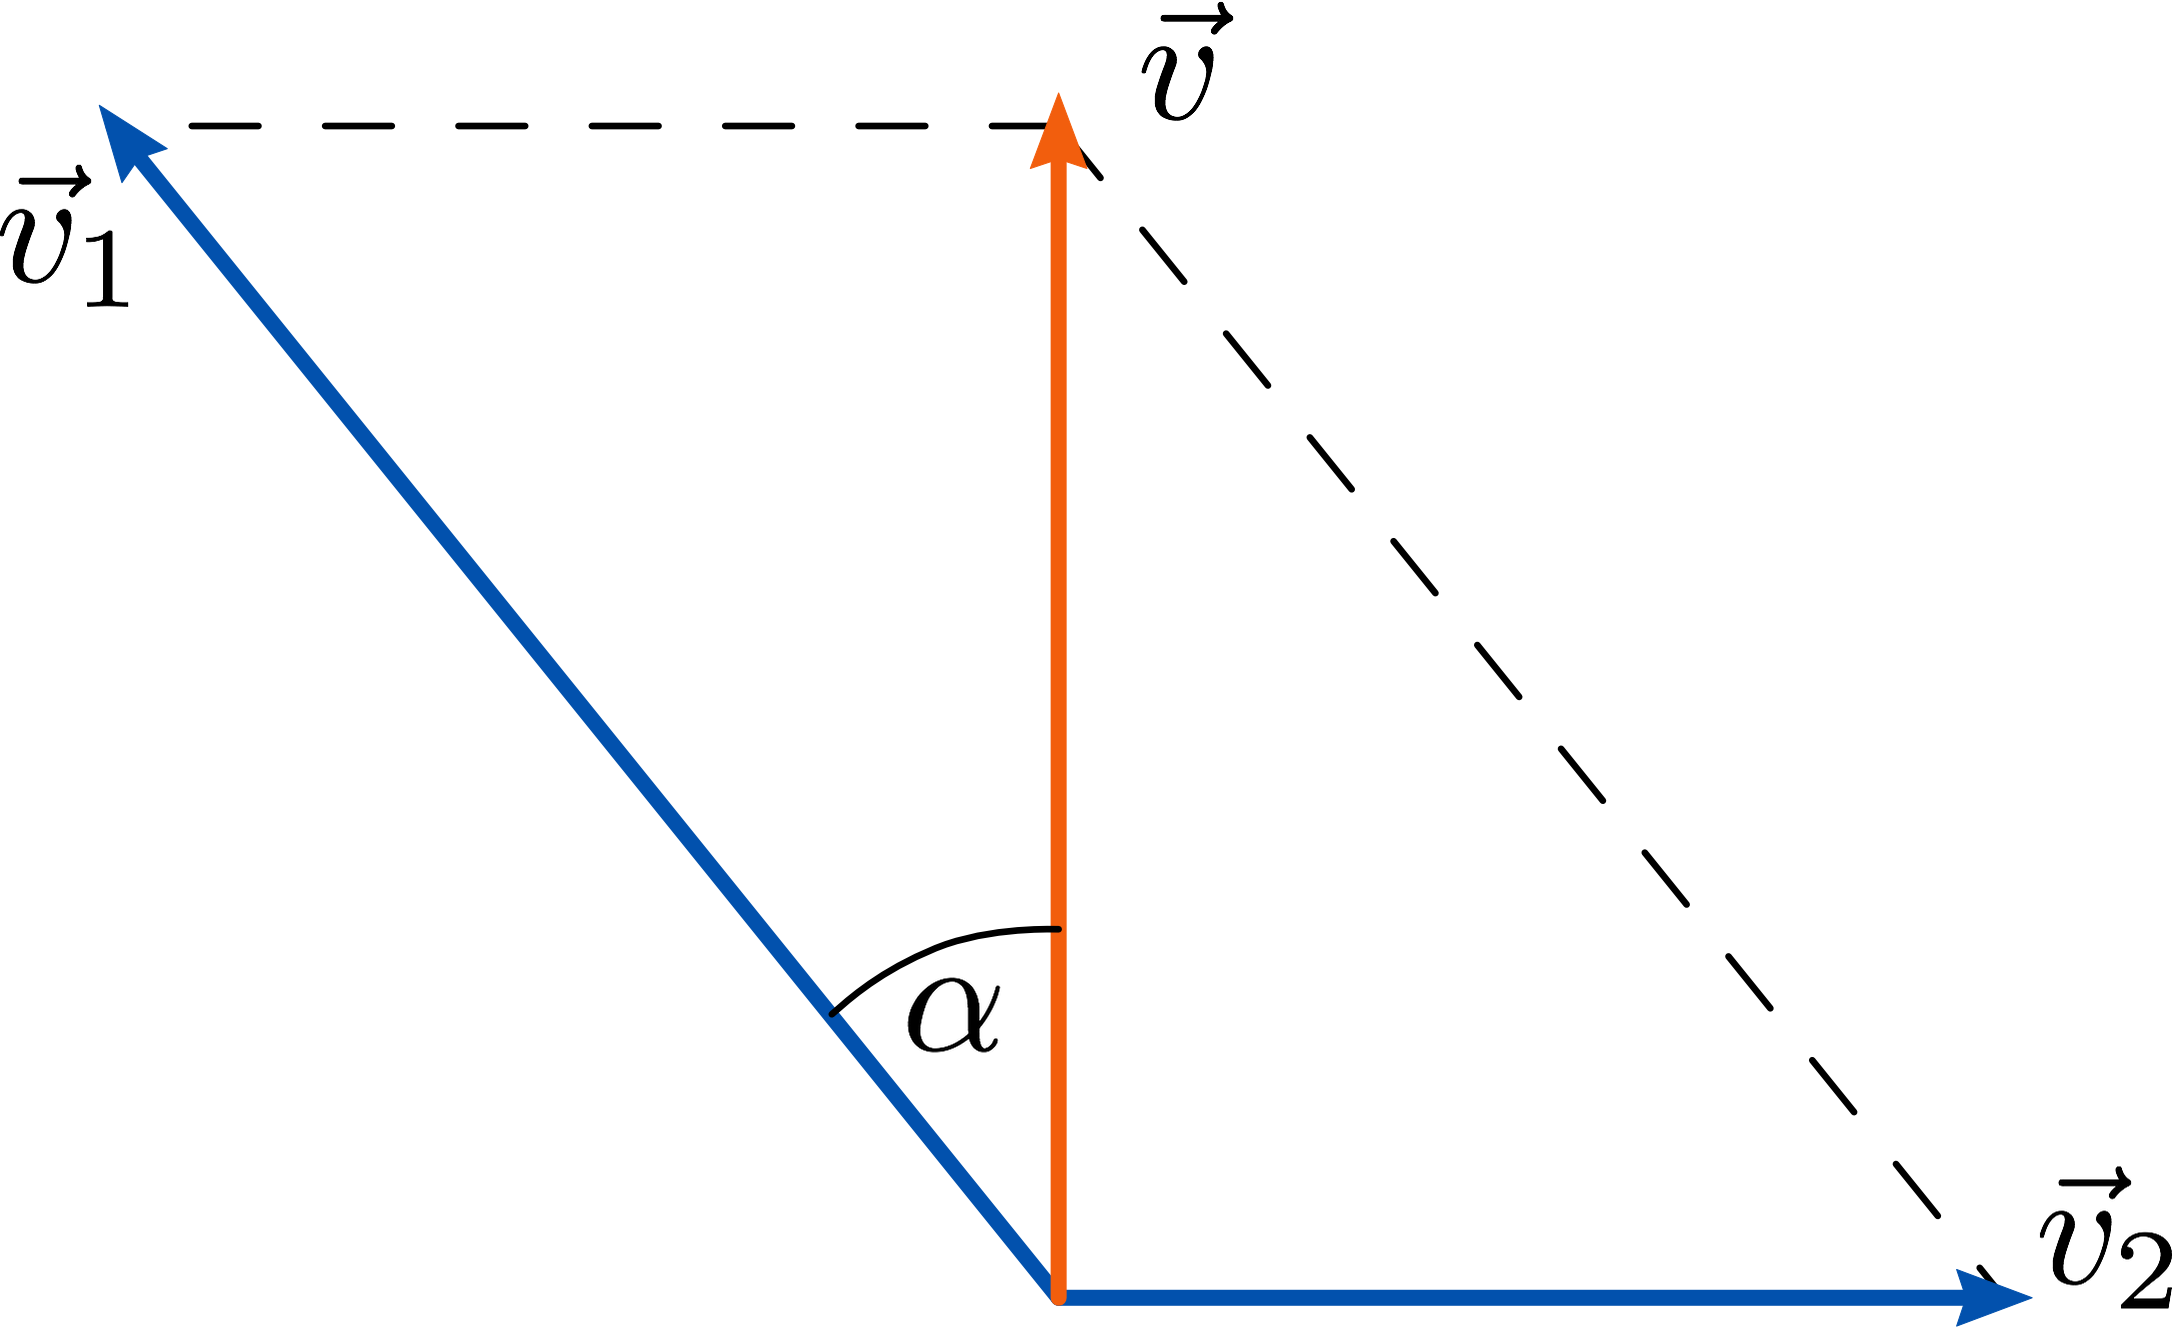
\includegraphics[width=0.45\textwidth]{dyn/exercises/vectoren_veerman}
% \end{figure}

De hoek vinden we dan als volgt (zie figuur):

\begin{align*}
\sin{\alpha} &= \frac{v_2}{v_1}\\
&\Downarrow\\
\alpha&=\bgsin\left(\frac{v_2}{v_1}\right)\\
&=38,7^\circ
\end{align*}

\end{oplossing}

\end{question}
\begin{question}
Hoeveel tijd heeft de veerman nodig om de overzijde te bereiken? 

\begin{oplossing}
De tijd nodig om de overzijde te bereiken vinden we door zijn snelheid loodrecht op de oever -- zijn resulterende snelheid $v$ -- te bekijken:
	\begin{align*}
		%v&=&v_1\cos{\alpha}\qquad\left(=v_1\cos\left(\bgsin\left(\frac{v_2}{v_1}\right)\right)=v_1\sqrt{1-\left(\frac{v_2}{v_1}\right)^2}=\sqrt{v_1^2-v_2^2}\right)\\
		%&\Downarrow&\\
		t=\frac{d}{v}=\frac{d}{\sqrt{v_1^2-v_2^2}}=96,1{\rm\,s}
	\end{align*}

\end{oplossing}
\end{question}
\end{exercise}

\begin{exercise}
	De coördinaten van een deeltje worden als functie van de tijd gegeven door
	\[
	\left\{
	\begin{aligned}
		x&=t^2 \\
		y&=t^2
	\end{aligned}
	\right.
	\]

	\begin{multipleChoice}
	\choice{Dan is de versnelling steeds evenwijdig aan de $x$-as.}
	\choice{Dan is de versnelling steeds evenwijdig aan de $y$-as.}
	\choice[correct]{Dan maakt de versnelling steeds een hoek van $45^\circ$ met de $x$-as.}
	\choice{Dan wordt het deeltje niet versneld}
	\end{multipleChoice}
\end{exercise}

\begin{exercise}
	De positie van een deeltje als functie van de tijd wordt beschreven door
	\[
	\vec{r}=bt\vec{e}_x+(c-dt^2)\vec{e}_y
	\]
	met $b=\SI{2,00}{\meter\per\second}$, $c=\SI{5,00}{\meter}$ en $d=\SI{1,00}{\meter\per\second\squared}$.
	
	\begin{question}
	Druk $y$ uit in functie van $x$. Hoe ziet de baan eruit?
	
	\begin{oplossing}
	We moeten dus de baanvergelijking geven. 
	Dit doen we door de tijd uit te drukken i.f.v. de positie $x$ en dit te substitueren in de coördinaatvergelijking $y(t)$.
	\begin{align*}
	x&=bt \quad \Leftrightarrow \quad t=\frac{x}{b}\\
	&\Downarrow\\
	y&=c-dt^2=c-\frac{d}{b^2}x^2
	\end{align*}
	Dit is een bergparabool met top $(0,c)=(0,\SI{5,00}{\meter})$.
	\end{oplossing}
	\end{question}
	
	\begin{question}
	Bepaal de snelheidsvector.
	
	\begin{oplossing}
	De componenten van de snelheid zijn:
	\begin{align*}
	v_x&=\frac{dx}{dt}=b\\
	v_y&=\frac{dy}{dt}=-2dt
	\end{align*}
	zodat de snelheid(svector) wordt gegeven door
	\begin{align*}
	\vec{v}&=v_x\vec{e}_x+v_y\vec{e}_y\\
	&=b\vec{e}_x-2dt\vec{e}_y
	\end{align*}
	\end{oplossing}
	\end{question}
	
	\begin{question}
	Op welk tijdstip ($t>0$) staat de snelheid loodrecht op de plaatsvector?
	
	\begin{oplossing}
	De rechte die de richting van de snelheid weergeeft, staat loodrecht op de rechte die de richting van de positievector weergeeft wanneer het product van de richtingsco\"effici\"enten gelijk is aan $-1$:
	\begin{align*}
	rc_{r}\cdot rc_{v}&=-1\\
	&\Updownarrow\\
	\frac{y}{x}\cdot\frac{v_y}{v_x}&=-1\\
	&\Downarrow\\
	\frac{c-dt^2}{bt}\cdot\frac{-2dt}{b}&=-1\\
	&\Downarrow \quad (t>0)\\
	t&=\sqrt{\frac{2cd-b^2}{2d^2}}\\
	&=1,73\rm\,s
	\end{align*}
	\end{oplossing}
	\end{question}
	
\end{exercise}
	


\begin{exercise}
	Een voorwerp maakt een beweging met volgende plaatscoördinaten:
	\[
	x=8t^{3},\qquad y=t^{6}-2,
	\]
	met \(x,y\) in \si{\meter} en \(t\) in \si{\second}.
	
	\begin{question}
	Bepaal de verplaatsing tussen \(t=\SI{0}{\second}\) en \(t=\SI{1}{\second}\).
	\end{question}
	
	\begin{question}
	Bepaal de snelheidsvector en de versnellingsvector op tijdstip \(t=\SI{1}{\second}\).
	\end{question}
	
	\begin{question}
	Is er op \(t=\SI{1}{\second}\) een tangentiële versnelling, een normale versnelling, of beide?% Licht kort toe welke componenten aanwezig zijn.
	\end{question}
	
	\begin{question}
		Bepaal de baanvergelijking van de baan van het voorwerp.
	%Bepaal de baanvergelijking (weg van \(t\)) van het projectiel: schrijf \(y\) uit in functie van \(x\).
	\end{question}
	
\end{exercise}

\begin{exercise}

 Vergelijk de begrippen \emph{verplaatsing} en \emph{afgelegde weg} met elkaar. Geef dus enkele gelijkenissen en enkele verschillen. 

 \begin{oplossing}
De twee begrippen hebben gemeen dat ze beide 
\begin{enumerate}
	\item een fysische grootheid zijn;
	\item een verandering in de positie beschrijven;
	\item als eenheid de meter hebben;
	\item een gelijke numerieke waarde voor de grootte hebben als de beweging in \'e\'en dimensie volgens eenzelfde zin plaatsvindt.
\end{enumerate}

Een verschil tussen de begrippen is

\begin{enumerate}
	\item dat de verplaatsing een vectorie\"ele grootheid is, daar waar de afgelegde weg een scalaire grootheid is. 
	\item dat de verplaatsing gedefinieerd is als het verschil tussen de eind- en de beginpositie ($\vec{\Delta r}=\vec{r}_2-\vec{r}_1$) en de netto verandering in de ruimte weergeeft terwijl de afgelegde weg de totaal aantal afgelegde meters gemeten langs de baan weergeeft. Het is de lengte van de route.
	\item dat de numerieke waarde van de grootte kan verschillen, ook als de beweging in \'e\'en dimensie plaatsvindt.
\end{enumerate}

\end{oplossing}

\end{exercise}

% 2d_abstract_1
\begin{exercise}

% !TEX root = ../main.tex




 De plaatsvector van een deeltje wordt (voor $t\geq0$) gegeven door
\begin{equation*}
	\vec{r}=-t\vec{e}_x+(t-1)^2\vec{e}_y
\end{equation*}
\begin{enumerate}
\item Geef de baanvergelijking.

\begin{oplossing}
	$y(x)=(x+1)^2$
\end{oplossing}

\item Wanneer is \'e\'en van de snelheidscomponenten nul?

\begin{oplossing}
	De snelheidscomponent volgens de $x$-as is nooit nul. Die volgens de $y$-as is nul wanneer: $2(t-1)=0$ oftewel wanneer $t=1$.
\end{oplossing}

\item Hoe groot is dan de snelheid?

\begin{oplossing}
	$v(1)=\sqrt{v_x^2(1)+v_y^2(1)}=\sqrt{(-1)^2+0^2}=1\,\text{s}$
\end{oplossing}

\item Waar is het deeltje dan?

\begin{oplossing}
	$\vec{r}(1)=-\vec{e}_x$
\begin{center}
\begin{tikzpicture}[line cap=round,line join=round,>=triangle 45,x=1cm,y=1cm]
\begin{axis}[
x=1cm,y=1cm,
axis lines=middle,
xmin=-3.2773087503908354,
xmax=1.9347255210454852,
ymin=-0.5305920286290815,
ymax=4.946070914425411,
xtick={-3,-2,...,1},
ytick={0,1,...,4},]
\clip(-3.2773087503908354,-0.5305920286290815) rectangle (1.9347255210454852,4.946070914425411);
\draw [samples=50,rotate around={0:(-1,0)},xshift=-1cm,yshift=0cm,line width=2pt,domain=-4:4)] plot (\x,{(\x)^2/2/0.5});
\end{axis}
\end{tikzpicture}
\end{center}
\end{oplossing}

\item Geef de versnellingsvector.

\begin{oplossing}
	$\vec{a}=2\vec{e}_y$, ($\vec{v}=-\vec{e}_x+2(t-1)\vec{e}_y$)
\end{oplossing}

\item Raakt de versnellingsvector aan de baan? Licht toe.

\begin{oplossing}
	Nee, de versnellingsvector is niet rakend aan de baan. Hij is altijd verticaal ge\"ori\"enteerd terwijl de afgeleide van de baanvergelijking ($y'=2(x+1)$) overal bestaat en dus nergens een verticale helling heeft.
\end{oplossing}

\end{enumerate}
\end{exercise}


% 2d_abstract_I_2
\begin{exercise}
	De coördinaten van een puntmassa veranderen als volgt:
	\begin{eqnarray*}
		x(t)=3t^2\qquad y(t)=2t^4
	\end{eqnarray*}
	\begin{enumerate}
		\item Bepaal de positie van het voorwerp na \SI{2,0}{s}.% en na $4,0\rm\,s$.
		\item Bepaal de vergelijking van de baan van het deeltje.
		\item Op welk ogenblik bedraagt de grootte van de snelheid \SI{10}{m/s}?
		\item Teken de snelheidsvector op de baan op dat ogenblik. Welke hoek maakt ze met de $x$-as?
	\end{enumerate}
	\begin{oplossing}
	\begin{itemize}
		\item[(a)] De plaatsvector op $t=\SI{2,0}{s}$ is $\vec{r}=12\,\vec{e}_x+32\,\vec{e}_y$.
		\item[(b)] De vergelijking van de baan vinden we door de parameter $t$ te elimineren uit de uitdrukkingen voor $x(t)$ en $y(t)$.
	\end{itemize}
	\begin{eqnarray*}
		x=3t^2\Leftrightarrow t^2&=&\frac{x}{3}\\
		&\Downarrow&\mathrm{substitutie}\\
		y&=&2t^4=2\left(\sqrt{\frac{x}{3}}\right)^4=\frac{2}{9}x^2
	\end{eqnarray*}
	Aangezien $x(t)$ niet negatief kan worden, is de baan een halve parabool.

	De grootte van de snelheid vinden we met stelling van Pythagoras, omdat we immers de componenten van de snelheid kunnen bepalen.
	\begin{eqnarray*}
		v(t)&=&\sqrt{v_x^2(t)+v_y^2(t)}\\
		&=&\sqrt{(6t)^2+\left(8t^3\right)^2}\\
	\end{eqnarray*}
	Om te weten wanneer die gelijk aan \SI{10}{m/s}, lossen we de volgende vergelijking op naar $t$.
	\begin{eqnarray*}
		10=\sqrt{(6t)^2+\left(8t^3\right)^2}&\Leftrightarrow&t=\pm 1
	\end{eqnarray*}
	Als we alleen positieve tijdstippen bekijken, houden we $t=\SI{1}{s}$ over. 

	De snelheidsvector is getekend in de figuur.
	% \begin{figure}[ht!]
	% \begin{picture}(390,160)(0,0)
	% \put(130,0){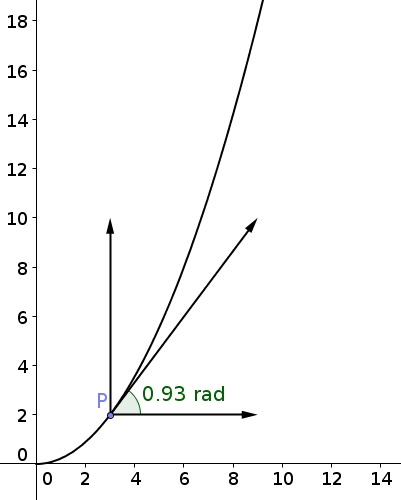
\includegraphics[width=0.3\textwidth]{dyn/exercises/12p53}}
	% \put(200,30){$\vec{v}_x$}
	% \put(200,65){$\vec{v}$}
	% \put(150,70){$\vec{v}_y$}
	% \put(205,120){$y(x)$}
	% \end{picture}
	% \end{figure}

	De hoek vinden we uit $\tan\alpha=\frac{v_y}{v_x}$ als $\alpha=\bgtan\!{\left(\frac{8}{6}\right)}=0,93\rm\,rad=\SI{55,13}{\degree}$.
	\end{oplossing}
\end{exercise}

\begin{exercise} De beweging van een voorwerp wordt beschreven door volgende coördinaatfuncties:
\begin{eqnarray*}
x(t)=5t+3\qquad y(t)=-4t^2+t
\end{eqnarray*}
\begin{enumerate}
%\item Bepaal de positie van het voorwerp na $2,0\rm\,s$ en na $4,0\rm\,s$.
\item Geef de verplaatsing tussen \SI{2,0}{s} en \SI{4,0}{s} en bereken haar grootte.
%\item Wat is de gemiddelde snelheidsvector tussen $2,0\rm\,s$ en na $4,0\rm\,s$?
\item Geef de ogenblikkelijke snelheid op \SI{2,0}{s}.
\item Geef de baanvergelijking.
\end{enumerate}

\begin{oplossing}
$\Delta\vec{r}=5(t_2-t_1)\vec{e}_x+(-4(t_2^2-t_1^2)+t_2-t_1)\vec{e}_y=10\vec{e}_x-46\vec{e}_y$

$||\Delta\vec{r}||=\sqrt{10^2+46^2}=2\sqrt{554}=\SI{47,07}{m}$

$\vec{v}=5\vec{e}_x+(-8t+1)\vec{e}_y$ zodat $\vec{v}(2)=5\vec{e}_x-15\vec{e}_y$

$y(x)=-4\left(\frac{x-3}{5}\right)^2+\left(\frac{x-3}{5}\right)=\frac{-4}{25}x^{2} + \frac{29}{25}x - \frac{51}{25}$

\end{oplossing}
\end{exercise}

\begin{exercise}
	Als $a_x=0$, wat weet je dan over de snelheid?
\end{exercise}

\end{document}
